\section{Testing of Format}
% This section meant to see if the template actually does the things

Figures will behave as Fig. \ref{fig: test}. Note that the placement may seem random, but is chosen by \LaTeX\ automatically.
\begin{figure}[!t]
\centering
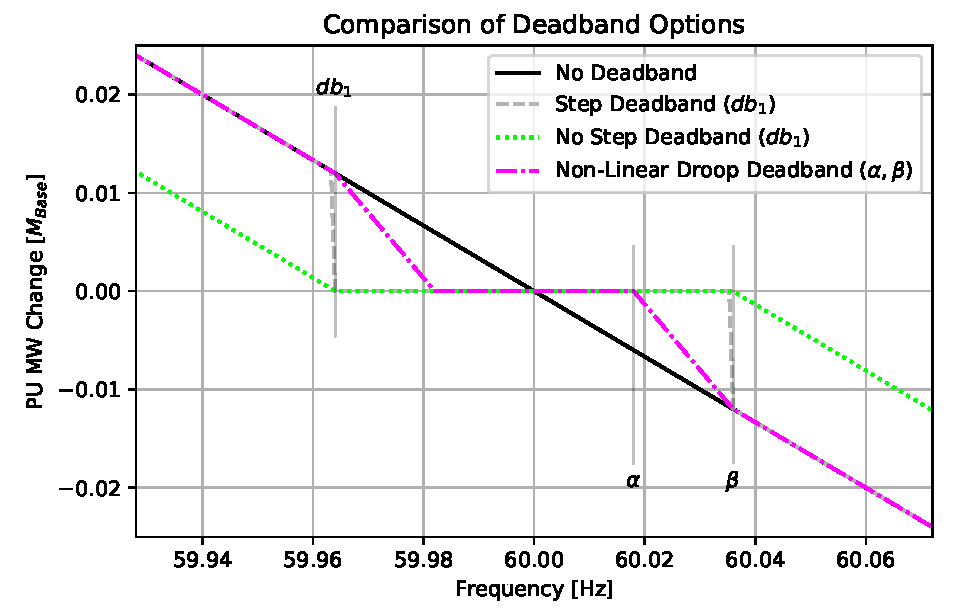
\includegraphics[width=\linewidth]{figures/dbAction3}
\caption{Testing of figure format.}
\label{fig: test}
\end{figure}


The default table example leaves something to be desired that is fulfilled by using the \verb|booktabs| package.
This is shown in Table \ref{tab: test2}.
% Testing of external table build for \input later
% Uses the IEEE table format guidelines
\begin{table}[!ht]
	\caption{Generic governor model parameters.}
	\label{tab: test2}
	\centering
	\begin{tabular}{@{} C{2cm} S[table-format=2.2] S[table-format=2.2] S[table-format=2.2] @{}} 	
		\toprule % @ signs to remove extra L R space
		\text{Parameter}	&	\text{Steam}	&	\text{Hydro}	&	\text{Gas}	\\		
		\midrule		
			Ts	&	0.04	&	0.40	&0.50\\
			Tc	&	0.20	&	45.00	&10.00\\
			T3	&	0.00	&	5.00	&4.00\\
			T4	&	1.50	&	-1.00	&0.00\\
			T5	&	5.00	&	0.50	&1.00\\
		\bottomrule
	\end{tabular}

\end{table}

References are only included if cited. For instance \cite{Kundur} or \cite{DonnellyVoltageControl} are randomly cited. Note that the sorting order is set to \verb|none|, which lists references in order cited.

Equations are entered as one may normally do in a \LaTeX\ situation and referenced as (\ref{eq: ACE}).
\begin{align}
\text{ACE}_{\text{tie line}} &= P_{gen} - P_{load} - P_{\text{sched interchange}}\\ \label{eq: TLace}
\text{ACE}_{\text{frequency bias}} &= 10B(f_{\text{actual}}-f_{\text{sched}})f_{base}\\
\text{ACE} &= \text{ACE}_{\text{tie line}} -\text{ACE}_{\text{frequency bias}} \label{eq: ACE}
\end{align}